
\chapter{Porting of image processing and computer vision algorithms}
The image processing and computer vision algorithms are computational intensive and has wide applications in defence, entertainment, digital security, etc. Thus, inorder to run these algorithms in real time, there is a need to be implement them in a platform like GPU. The objective of this chapter is to implement the algorithms adaptive contrast enhancement and motion de-blur on NVIDIA GeForce GT640 GPU and analyse the speed performance with respect to the Intel i5 CPU@3.0GHz.
\section{Automated Ground Comtrol System(AGCS)} 
The Figure \ref{Hies target hardware} shows the list of different hardware components connected together to form a High-performance computing platform. The Single Board Computer (SBC) acts as a master and other hardware works in conjunction with SBC as slaves. AGCS follows a typical client-server architecture, as shown in Figure \ref{Hies target hardware}. In this work, Adaptive contrast enhancement and motion de-blur algorithms are ported onto to GPGPU to accelerate the execution time.
\begin{figure}[h!]
	\centering
	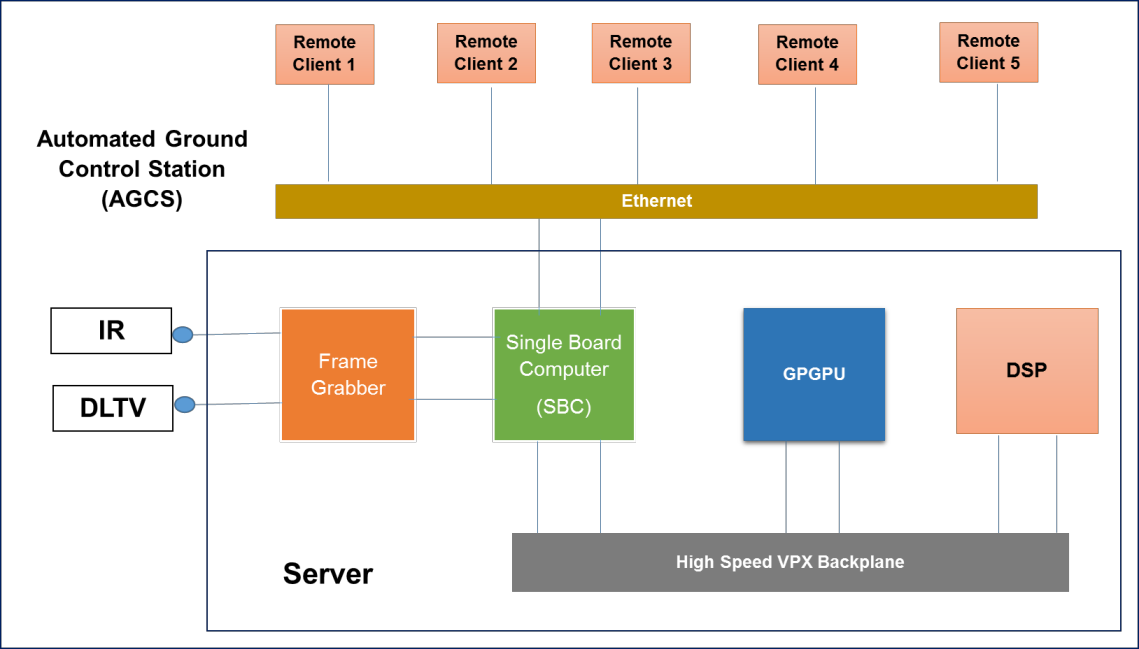
\includegraphics [width=\linewidth]{TargetHardwareHIES.png}
	\caption{The different hardware components in automated ground control system}
	\label{Hies target hardware}
\end{figure}
\section{Adaptive contrast enhancement algorithm \cite{ACE}}
Contrast enhancement is used to increase the contrast of an image for better visual appearance. Histogram equalization can perform contrast enhancement, however it also enhances the noise in the image.  So adaptive contrast enhancement algorithm is being used to avoid the noise component amplification \cite{ACE}.
\subsection{Algorithm flow}
This subsection presents the details of the adaptive contrast Enhancement algorithm as shown in Figure \ref{ACE} . In this work, adaptive contrast Enhancement algorithm is implemented on GPGPU computing. 
\begin{itemize}
\item{\textbf{Step 1:}} In this step, the RGB color image is converted into HSV colour model. The H, S and V components can be computed using the Equations \ref{Heq}, \ref{Seq} and \ref{Veq} respectively. In the case of YUV color model images, only Y component is sufficient to process.
	
	\begin{equation}\label{Heq}
		H=
		\begin{cases}
		\text{undefined}, & \text{if}\ max=min \\
		60^o \times \frac{g-b}{max-min}+0^o, & \text{if} max= r \&\& g\geq b \\
		60^o \times \frac{g-b}{max-min}+360^o, & \text{if} max= r \&\& g < b \\
		60^o \times \frac{b-r}{max-min}+120^o, & \text{if} max= g \\
		60^o \times \frac{r-g}{max-min}+240^o, & \text{if} max= b \\
		\end{cases}
	\end{equation}
	\begin{equation}\label{Seq}
	S=
	\begin{cases}
	0, & \text{if}\ max=0 \\
	\frac{max-min}{min} \times 255, & \text{otherwise}
	\end{cases}
	\end{equation}
	\begin{equation}\label{Veq}
	V = max \times 255	
	\end{equation}
	where $r,g,b$ are red, green and blue components in the image. $max$ is the maximum value among the three ($r,g,b$) components.
	\item{\textbf{Step 2:}} In this step, the histogram $H_v(x_k)$ for the V component (Y component in case of YUV image) is calculated. where $x_k$ represents the \textit{kth} brightness level and $n_k$ is the pixels count in the image having brightness level $x_k$.
	\begin{equation}\label{histeq}
		H_v(x_k)=n_k
	\end{equation}
		The luminance histogram is smoothed by convolving gaussian kernel \cite{ACE} with the luminance histogram $H_v(x_k)$. The smoothing operation is given as
		\begin{equation}\label{gausseq}
		\begin{split}		
		S_{HV}(x,\sigma_g)&=H_v(x)*g(x,\sigma_g)=\int_{-\infty}^{\infty} 	H_v(u)g(x-u,\sigma_g)du\\
		&=\int_{-\infty}^{\infty} 	H_v(u) \frac{1}{\sqrt{2\pi\sigma_g}} \exp^\frac{(x-u)^2}{2{\sigma_g}^2}
		\end{split}
		\end{equation}
		where $\sigma_g$ is the standard deviation and $S_{HV}(x,\sigma_g)$ is the smoothed histogram.
		
		\paragraph*{}The average difference is calculated between the consecutive values ($x_{k-1}, x_{k+1}$) in the luminance histogram. In the average difference, the positive to negative crossover gives a peak($p$) while the negative to positive crossover gives a valley($v$). The avergae difference operation is given as
		\begin{equation}\label{smootheq}
		S_{HV}(x)=\frac{1}{\sigma_g - 1}\sum_{i=1}^{\sigma_g - 1}\frac{S_{HV}(x+i)-S_{HV}(x-i)}{2\times i}
		\end{equation}
		\item{\textbf{Step 3:}} At this step, the automatic and parameter free piece-wise linear transformation(APFPLT) for $k-1$ line segments is calculated betweeen input parameters ($v_k$) and output parameters($y_k$) \cite{ACE}. The APFPLT is given as,
		\begin{equation}\label{PLTeq}
			T_{k-1} =\frac{(y_k-y_{k-1})}{x_k-x_{k-1}} \times {(x-x_{k-1})} +y_{k-1}
		\end{equation}
		In piece-wise linear transformation (PLT), $k$ input parameters and $k$ output parameters are need to set manually for $k$ luminance distributions. Whereas, in APFPLT the valleys \{$v_0,v_1,v_2,...,v_k$\} are used for input parameters, and the output parameters are calculated as, 
		\begin{equation}\label{probeq}
			y_k = \sum_{x=s}^{v_k} Pr(x) \times 255	
		\end{equation}  
		The $Pr(x)$ is the probability of the luminance distribution and $s$ is the start luminance of the input image.
		\item {\textbf{Step 4:}} At this stage, the HSV model image is converted into rgb colour model image \cite{ACE}. 
\end{itemize}

\begin{figure}[htb]
	\centering
	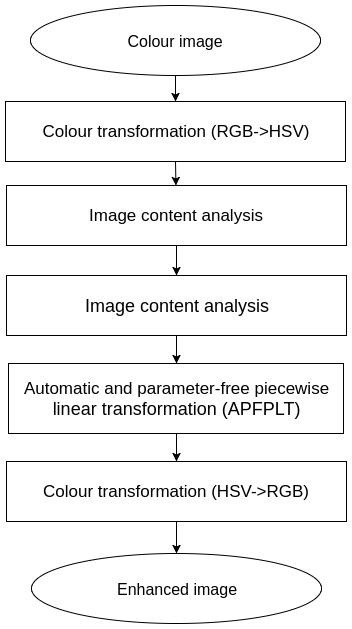
\includegraphics[width=0.5\linewidth]{ACEblockdiagram.png}
	\caption{Adaptive contrast enhancement algorithm flow}
	\label{ACE}
\end{figure}
\subsection{GPGPU implementation}
The adaptive contrast enhancement algorithm is implemented on a CPU-GPU platform with Intel i5 CPU@3.0GHz and NVIDIA GeForce GT640 GPU with 384 CUDA cores,
\begin{itemize}		
		\item{\textbf{Step 1:}} The HSV conversion is not implemented on GPU, since a standard software library is used.
		\item{\textbf{Step 2:}} This step analyses the image content, the GPU implementation of the substeps are shown below.
		\begin{itemize}
			\item The histogram contains 255 levels as the pixel intensities. Thus, all the pixels in the image contributes to 255 histogram levels. In GPU, if a single thread operates on a pixel, then image size number of threads updates only 255 outputs. It means that one or more threads tries to update a single output. A thread block of 32x32 size is selected which has given good speed up. For an image of size 640x480, a grid of 20x15 blocks is created to complete the histogram calculation.	
			\item The histogram smoothing and the remaining oprations in image content analysis are implemented in GPU with single thread, since these are sequential in nature and dependent on other outputs.			
		\end{itemize}
		\item{\textbf{Step 3:}} After having the required information, the PLT is implemented on GPU with full parallelism. From the equation \ref{PLTeq}, the PLT operation is independent of other outputs. The output size number of threads can concurrently work to compute all the outputs. A thread block configuration explained for histogram calculation is also used here.
		 \item{\textbf{Step 4:}} The HSV model to rgb model image conversion is not implemented on GPU, since a standard software library is used.
\end{itemize}
\subsection{Results and discussions}
The adaptive contrast enhancement algorithm is implemented in a system with Intel i5 CPU @3.0GHZ and NVIDIA GeForce GT640 GPU with 384 CUDA cores.The speed performance is analysed by considering different images with varied resolutions. Initially the algorithm is implemented on a system with Intel i5 CPU @3.0GHZ then the same algorithm is implemented in a CPU-GPU platform with Intel i5 CPU @3.0GHZ and NVIDIA GeForce GT640 GPU. The execution times are tabulated in the Table \ref{timing of ace}, it also tabulates the speed up of algorithm. The speed up calculated as the ratio of CPU timing to the CPU-GPU timing.\paragraph*{} From the table it is observed that the CPU-GPU implementation runs faster than the CPU only implementation. The speed up is increased as the image resolution is increased and is saturated at the end. The saturation might be due to the increased number of valleys($v$) in the image content analysis. 

\begin{figure}[htb]
\centering
\subfloat[input]{{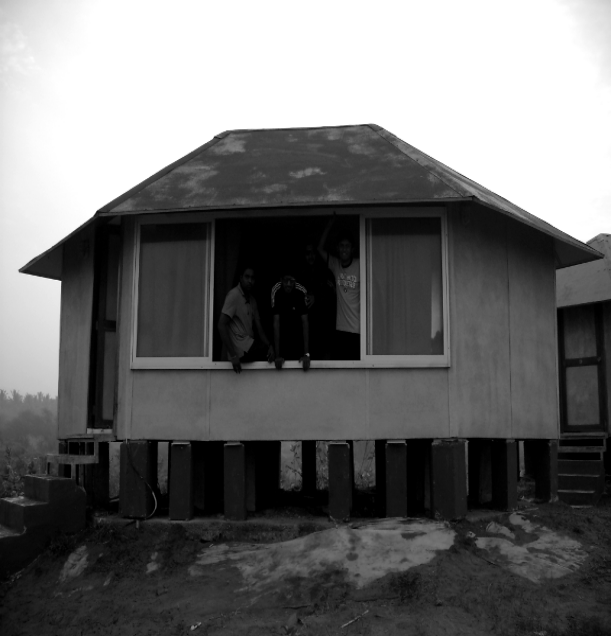
\includegraphics[width=6cm]{aceinput.png} }}%
\qquad
\subfloat[output]{{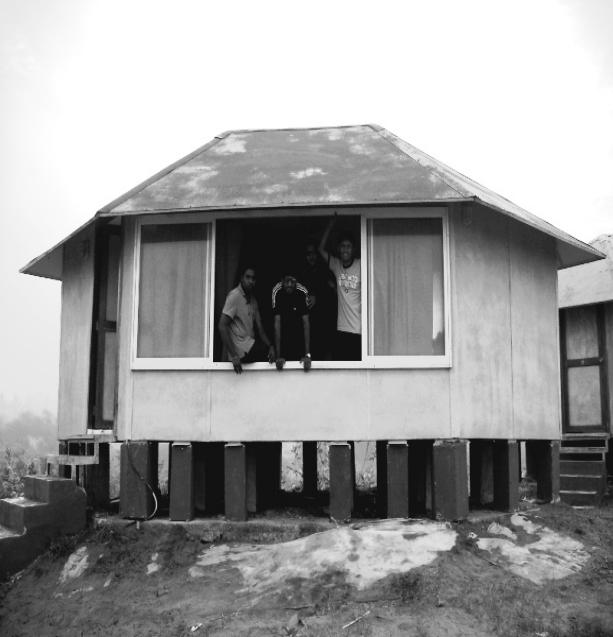
\includegraphics[width=6cm]{aceoutput.png} }}%
\caption{Adaptive contrast enhancement functional results}%
\label{fig:ace results}%
\end{figure}
\begin{table}[htb]
\centering
\begin{tabular}{ |c|c|c|c| }
\hline
\textbf{Image Resolution} & \textbf{CPU(in ms)} &  \textbf{GPU(in ms)} & \textbf{Speed Up}\\
\hline
640 X 480 & 18.73 & 3.23 & 6x \\
\hline
1280 x 720 & 55.27 & 6.17 & 9x \\
\hline
1920 x 1080 & 104.54 & 11.74 & 9x \\
\hline
\end{tabular}
\caption{Timing performance of Adaptive contrast enhancement algorithm.}
\label{timing of ace}
\end{table}
\section{Motion de-blur algorithm \cite{BlurredImageRestoration} \cite{motionBlurEstimation}}
Restoration of blurred images is useful in consumer-level photography, medical imaging and astronomy. One of the reasons for the Blur in an image is due to the motion of the camera and is called the motion blur. Motion blur in images happens when there exist a relative motion between the camera and an object. Blur distorts the details in the image. The original image can be restored from the blurred image, if we can estimate the blur kernel. The blur kernel estimation depends on the blur motion and blur direction in the blurred image. Deconvolving blurred image with the blur kernel gives the original image. This process of Image restoration is called de-blurring. The deblurring methods are categorised based on the deconvolution used. The deconvolution methods available for deblurring are non-iterative Weiner algorithm \cite{BlurredImageRestoration} and iterative Lucy-Richardson, sparse method, etc. In this work sparse deconvolution is used.
\subsection{Algorithm Flow}
In the following, the algorithm flow of Motion De-blur is explained with references. In this work, high performance implementation of this algorithm is designed to get best performance using GPGPU computing. The algorithm flow is shown in the Figures \ref{blur angle}, \ref{blur length} and \ref{deconv} The motion de-blur algorithm is split into two parts as shown below for simplifying the explanation.
\begin{enumerate}
	\item Blur kernel estimation
	\item Deconvolution 
\end{enumerate}
\subsubsection{Blur kernel estimation}
In finding blur kernel there are three stages, Blur angle calculation, blur length calculation and estimating the blur kernel. 

	\begin{itemize}
	\item \textbf{Blur angle calculation} \hfill \break For calculating the blur angle following are the  steps implemented.%\hfill \newline	
	\par \textbf{Step 1: Gradient of the Image} \hfill \newline	
	Gradient gives the edge information of the image. These image edges contains the useful information about the blur parameters \cite{BlurredImageRestoration}. The gradient of the image can be calculated as
		\begin{equation}
		G_a=\frac{f(a+1,b) - f(a-1,b)}{2}
		\end{equation}
		\begin{equation}
		G_b=\frac{f(a,b+1) - f(a,b-1)}{2}
		\end{equation}
		\begin{equation}\label{gradeq}
		G = \sqrt{{G_a}^2+{G_b}^2}
		\end{equation}

	\vspace{0.2cm} \par{}From the equation \ref{gradeq} the image gradient $(G)$ is the magnitude of horizontal$(G_a)$ and vertical gradient$(G_b)$. For an image of size $N\times M$, $f(a,b)$ represents the image intensity at location $(a,b)$, where $a$ varies from $1,.....,N$ and $b$ varies from $1,....,M$.
	
	\par\textbf{Step 2: Power spectrum calculation} \hfill \\
	The power spectrum of the image gradient contains a regular structure which has a relationship with the blur length and blur angle \cite{BlurredImageRestoration}.
	\paragraph*{} The 2-Dimensional Discrete Fourier Ttransform can be calculated as,
	\begin{equation}\label{pseq}
	F(u,v)=\sum_{a=1}^{N}\sum_{b=1}^{M}f(a,b) \exp^{\omega_N (a-1)(u-1)} \exp^{\omega_M (b-1)(v-1)}
	\end{equation}
	where $\omega_M=-\frac{2\pi i}{M}$, $\omega_M=-\frac{2\pi i}{N}$ and $F(u,v)$ represents the output spectrum.
	\par \textbf{Step 3: Bandpass Filtering} \hfill \break
	 The band-pass Butterworth filter can be designed by cascading two Butterworth filters, a Low pass and a High pass. First, a Low pass filtering is done on the input and then a High pass filtering follows. The discrete form of Butterworth low pass filter can be calculated by using the Equation \ref{bwfeq}. 		
	\begin{equation}\label{bwfeq}
	G\big(u,v) = \frac{1}{\big(1+\big(\frac{D(u,v)}{d}\big)^{2 n}\big)}
	\end{equation}

	 \par\noindent \vspace{0.2cm}
	\begin{equation} \label{dist}
	D(u,v)=\sqrt{(u-M/2)^2+(u-N/2)^2}
	\end{equation}
	where variable $D(u,v)$ is the operating frequency, $d$ is the cut-off frequency, $n$ is the order of the filter and $N,M$ are width and height of the image respectively.

	\par \textbf{Step 4: Radon Transform} \hfill \break
	The Radon transform operates on the filtered power spectrum. It finds the parallel stripes from the pattern contained in the power spectrum. These parallel stripes contains the useful information regarding the blur angle \cite{BlurredImageRestoration}. The Radon transform finds the projections of the data for a given angle as expressed in Equation \ref{radoneq}. The Radon transform will be found for selected several angles. The angle at which maximum occcurs in the Radon transform output gives the blur angle.
	\begin{equation}\label{radoneq}
	R_\theta(x')=\sum_{-\infty}^{\infty} f(a'\cos\theta-b'\sin\theta,a'sin\theta + b'\cos\theta)
	\end{equation}
	where 
	$\begin{bmatrix}
		a'\\
		b'\\
	\end{bmatrix} = \begin{bmatrix}
	cos\theta & sin\theta \\
	-sin\theta & cos\theta
	\end{bmatrix}$ 
	 where $a$ represents x-axis co-ordinate and $b$ represents y-axis co-ordinate.
\begin{figure}[h!]
	\centering
	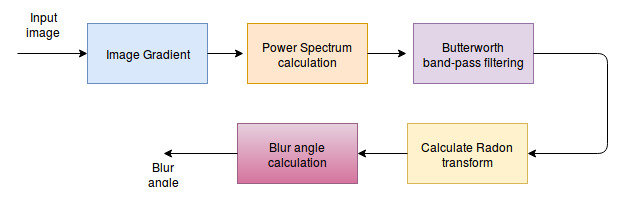
\includegraphics[width=\linewidth]{blur_angle_md.jpg}
	\caption{Block-diagram for calculating blur angle in motion de-blur algorithm}
	\label{blur angle}
\end{figure}
\item \textbf{Blur length calculation}\hfill \break For calculating the blur length following are the steps implemented. 
	\par \textbf{Step 1: Estimate the Target function} \hfill \break
	The spatial domain image is converted into the spectral domain and a log transform is applied, which is then converted back to the spatial domain. The spatial domain data is rotated with the estimated blur angle, a vector is formed by averaging all the columns in the rotated data \cite{BlurredImageRestoration}. This vector is called target function which contains the information regarding the blur length.
	\par \textbf{Step 2: Blur length calculation from the target function} \hfill \break
	The target function, shown in the Figure \ref{target function} illustrates the blur length calculation. The distance $d$ has inverse relationship with the blur length. For an image of MxM size, the blur length can be calculated as,
	\begin{equation}\label{blurlengtheq}
		Blur length = \frac{M}{d}
	\end{equation}
	\begin{figure}[h!]
		\centering
		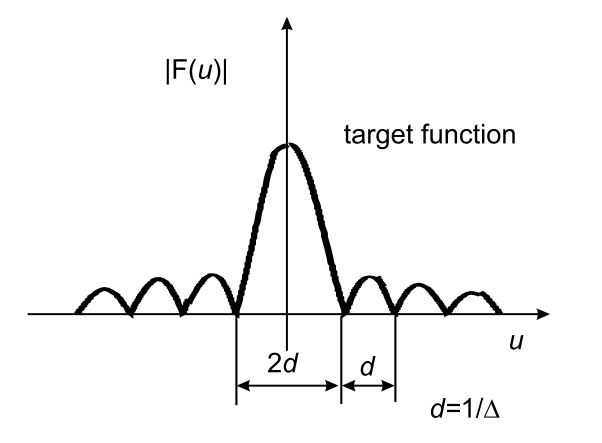
\includegraphics[width=0.5\linewidth]{targetFun.png}
		\caption{Target function for calculating blur length in motion de-blur algorithm \cite{ACE}}
		\label{target function}
	\end{figure}
	\begin{figure}[h!]
		\centering
		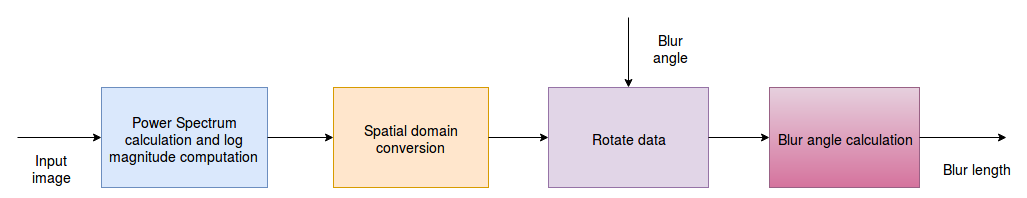
\includegraphics[width=\linewidth]{blur_length_md.png}
		\caption{block-diagram for Calculating blur length in motion de-blur algorithm}
		\label{blur length}
	\end{figure}
	\item \textbf{Estimating the Blur kernel} \hfill \break
	With the known blur length and blur angle the blur length can be estimated \cite{BlurredImageRestoration}. Since the generation of blur kernel takes a less time on CPU, so it is not a targeted portion for parallel implementation.
\end{itemize}
\subsubsection{Deconvolution}
The deconvoluton of blurred image with the estimated blur kernel gives the de-blurred image. In this algorithm sparse method based deconvolution is used. It contains a series of convolutions with the static kernels(Kernel1, Kernel2, Kernel3 and Kernel4) and blur kernel. The static kernels are defined as,\par\noindent
Kernel1 = [-1,1] \par\noindent
Kernel2 = [-1,-1] \par\noindent
Kernel3 = [-1,2,-1] \par\noindent
Kernel4 = [-1,1,1,-1]
\begin{itemize}
\item Three types of convolutions such as same,valid and full are used \cite{BlurredImageRestoration}. Same convolution yields the output with size equal to the input dimensions. The same type of convolution is shown in the Figure \ref{fig:convolution}. The general discrete convolution operation is given as,
\begin{equation}\label{conveq}
\begin{split}
	h(n)&=f(n)*g(n) \\
	&=\sum_{m=-M}^{M} f(n-m)g(m)
\end{split}
\end{equation}
\item The valid type of convolution yields only the valid pixels, i.e at pixels where there are insufficient pixels surround to form a window are avoided to calculate output.
\item For valid type of convolution an image of size 682x482 and with a kernel of size 3x3, the output is 640x480. The output size here can be computed by using the kernel size. In valid convolution for a 3x3 kernel, the output size in every dimension is reduced by 2 (kernel size in x direction-1).
\item The full convolution gives the padded output. For an image of 640x480 with a convolution kernel axb, the output size in x direction is 640+a-1 and in y direction is 480+b-1.
\end{itemize}
\begin{figure}[h!]
	\centering
	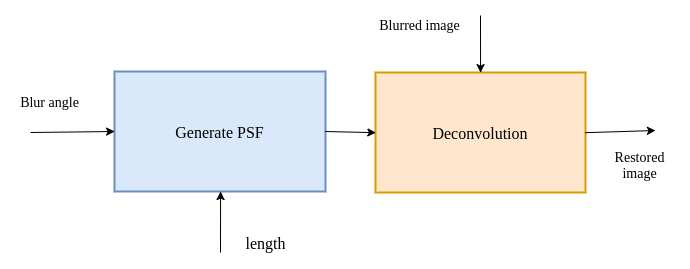
\includegraphics[width=\linewidth]{ImageRestorationMD.png}
	\caption{Image restoration}
	\label{deconv}
\end{figure}

\begin{figure}[h!]
	\centering
	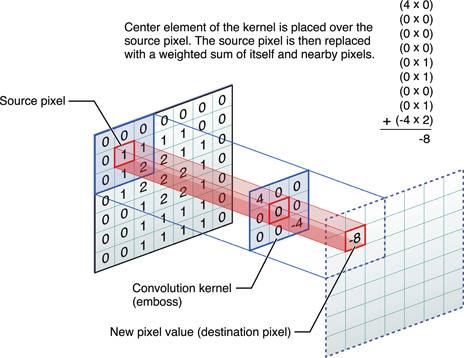
\includegraphics[width=0.75\linewidth]{kernel_convolution.jpg}
	\caption{Convolution operation that gives the output with size equal to input \cite{convolution}}
	\label{fig:convolution}
\end{figure}
\subsection{GPGPU implementation}
The motion de-blur algorithm has two stages as explained in the algorithm flow. Blur kernel estimation and deconvoution. These two stages are implemented in GPU as below,

\subsubsection{Estimating blur kernel}
The blur kernel estimation has three stages as explained in the algorithm flow. Blur angle estimation, blur length calculation and blur kernel generation. These stages are analysed for GPU implementaton. The blur angle calculation and blur length calculation are taking considerable time for execution on CPU and is a targetted portion for GPU implementation. The blur kernel generation takes less time and don't qualify for GPU implementation. The blur angle calculation is implemented on GPU as below.

\begin{itemize}	
	\item \textbf{Blur angle calculation} \hfill \break
	The blur kernel estimation has several steps, such as Gradient of the image, power spectrum calculation, butter worth bandpass filtering and Radon trnsform. These steps need to be parallelized to implement on GPU. 
	\par \textbf{Gradient of the image} \hfill \break
	\begin{itemize}

	\item The horizontal gradient at $(a,b)$ works on the next pixel $(a+1,b)$ and previous pixel $(a-1,b)$ in a row, as in Equation \ref{gradeq}. The vertical gradient at $(a,b)$ works on next pixel $(a,b+1)$ and previous pixel $(a,b-1)$ in a column. These two gradients are used to find the final gradient as in equation \ref{gradeq}.
	\item In GPU, a single gradient output can be calculated by a single thread. The output size number of threads can compute all the outputs in parallel. The pixel co-ordinates are mapped to thread indices.

	\item As shown in Figure \ref{fig:imgradient}, a block of threads with size 16x8 is proposed for computing gradient. This block configuration has given good speed up unlike other configurations. The grid size in the GPU can be calculated as,\\
	\begin{equation}\label{grid-blockeq}
	\begin{split}
		\text{grid dimension in  x direction} &= \text{image width}/\text{block dimension in x direction} \\
		\text{grid dimension in  y direction} &= \text{image height}/\text{block dimension in y direction}
	\end{split}
	\end{equation}
	\item For an image of size 640x480 , a grid of size 40x60 is created to compute all the gradient outputs.	
	\begin{figure}[h!]
		\centering
		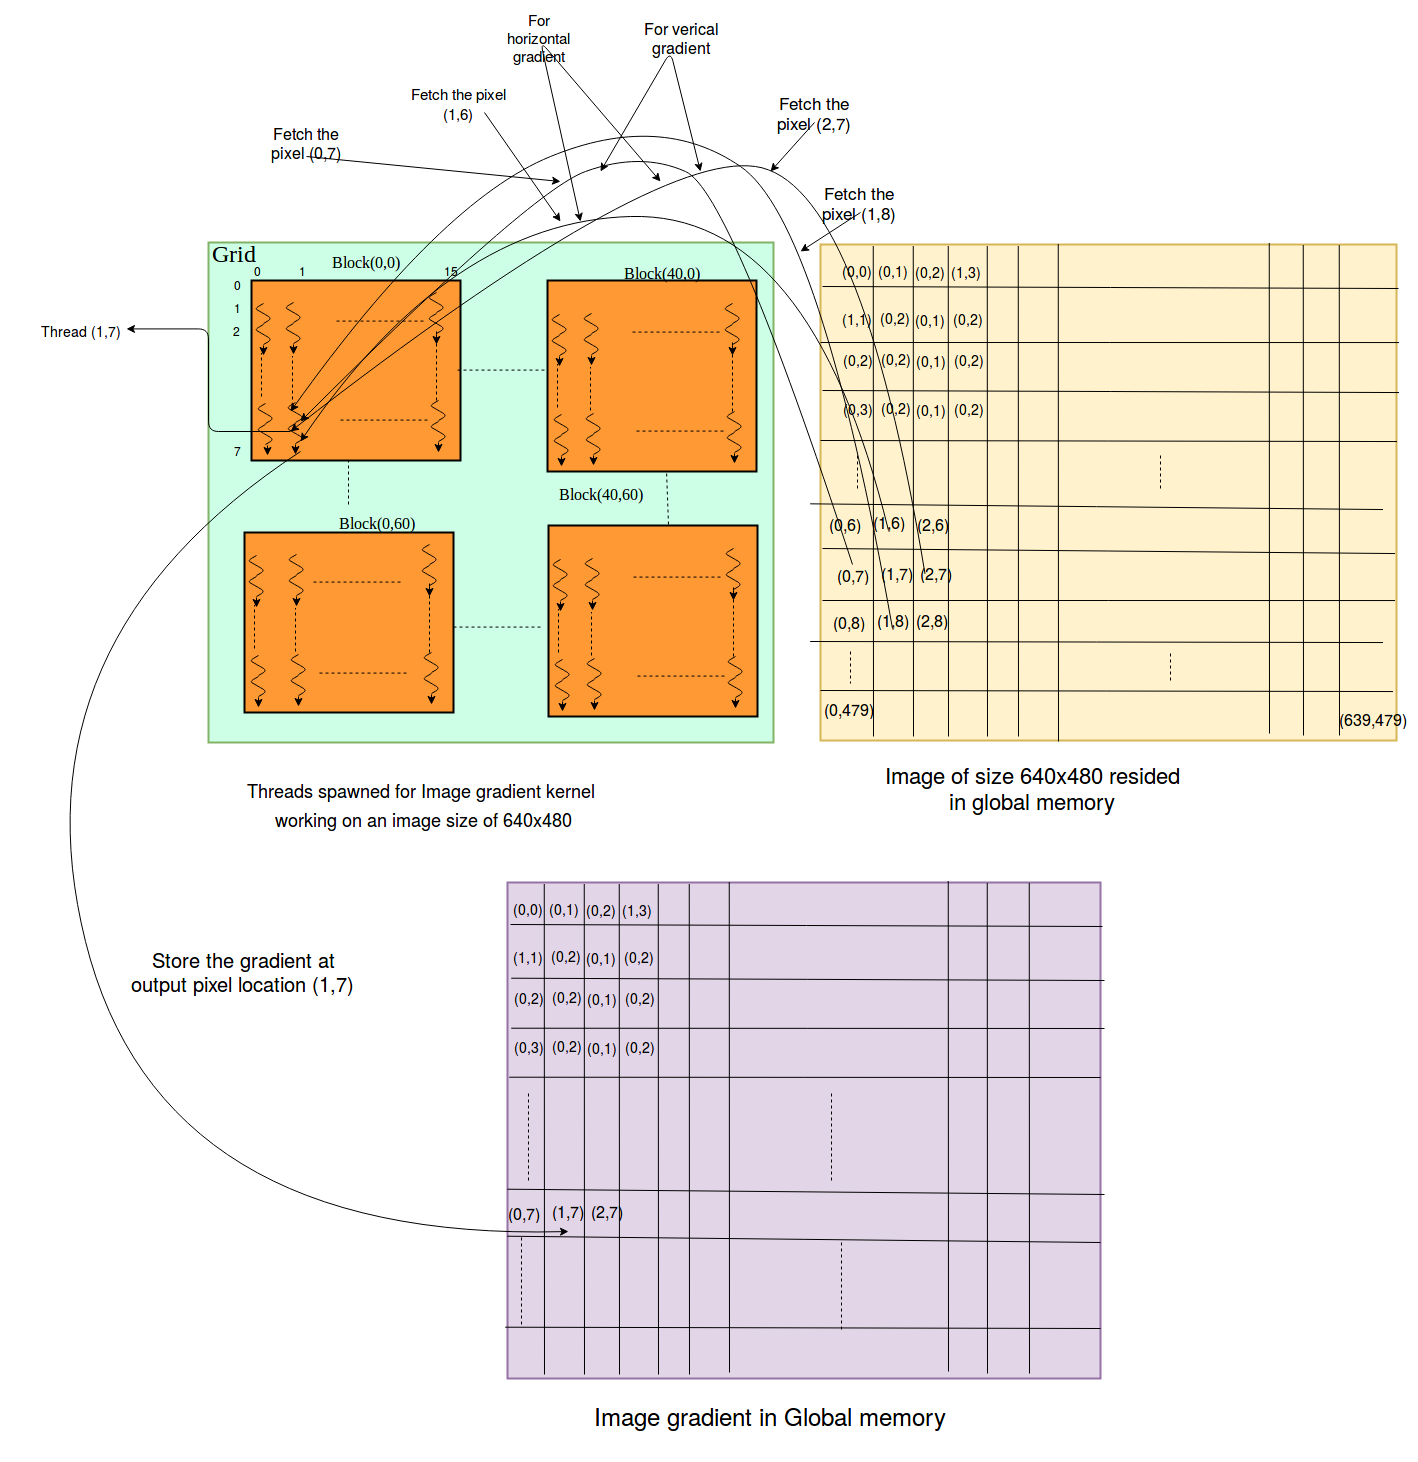
\includegraphics[width=\linewidth]{imageGradient.png}
		\caption{Thread access pattern for a kernel which finds image gradient on a image of size 640x480}
		\label{fig:imgradient}
	\end{figure}	
\end{itemize}
	\item \textbf{Power spectrum of the image gradient}
\begin{itemize}
	\item Power spectrum calculation in Equation \ref{pseq} is implemented using a standard CUDA library \textit{cufft}.
\begin{figure}[h!]
		\centering
		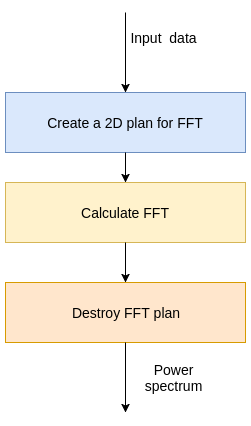
\includegraphics[width=0.4\linewidth]{powerSpectrumCalculation.png}
		\caption{CUDA cufft library usage for calculating FFT}
		\label{fig:cufft}
\end{figure}
	\item The power spectrum calculation is explained in the Figure \ref{fig:cufft}. 
\end{itemize}
\item \textbf{Butterworth bandpass filtering}
\begin{itemize}
	\item In this operation first a low pass filter is applied on the spectrum with a cut-off digital frequency of 3 ($d$). Then high pass filter is applied on the spectrum with cut-off digital frequency($d$) of 2. Both the filters are joined to form a band pass filter.
	\item From the Equation \ref{bwfeq}, the operating digital frequency $D(u,v)$ is calculated using the pixel location, as in Equation \ref{dist}. 
	\item Each output produced in the filtering is independent of the other output. An output at (a,b) can be produced with a thread at (a,b) in the grid.
	\item As shown in the Figure \ref{fig:butterworth}, for a spectrum of 640x480 the output is also of same size. A block with 16x8 threads is selected randomly and is found to be efficient, and a grid of 40x60 is formed to compute all the outputs.
\end{itemize}
\begin{figure}[h!]
	\centering
	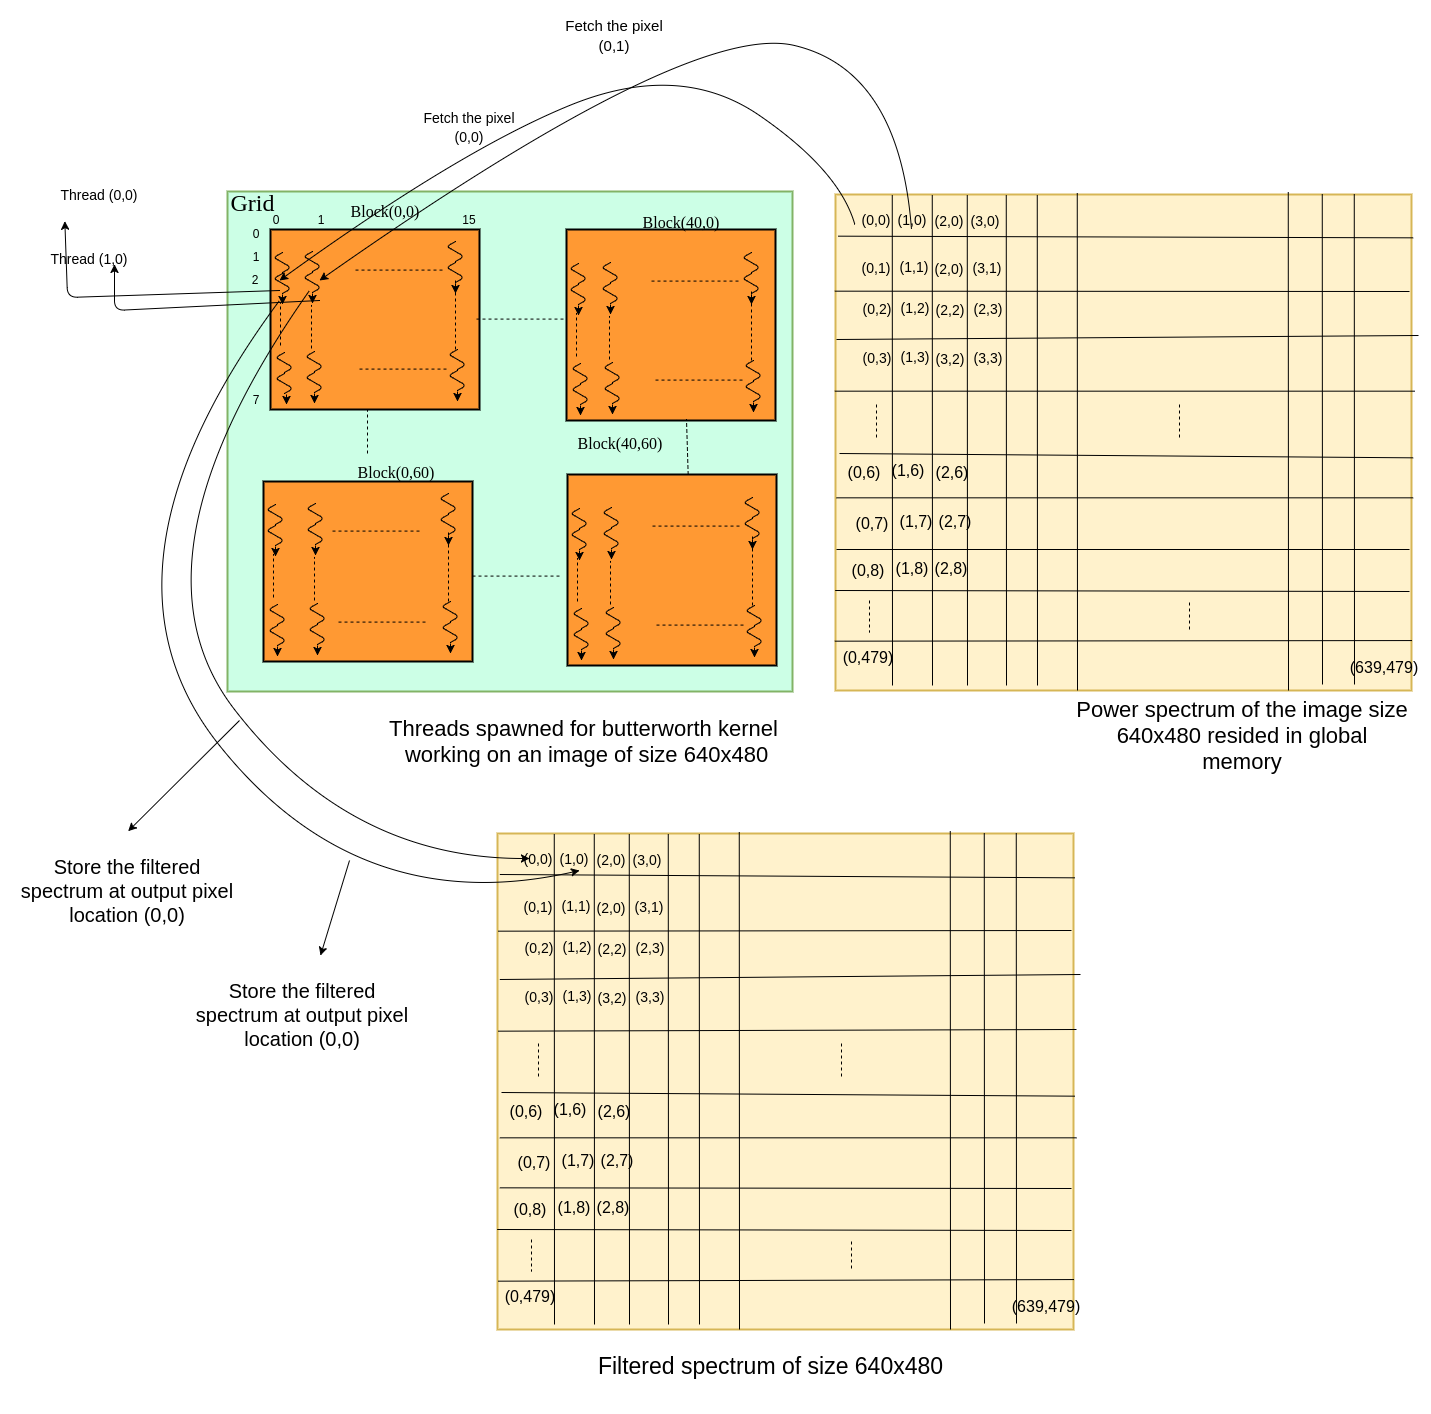
\includegraphics[width=\linewidth]{ButterworthFiltering.png}
	\caption{CUDA kernel for Butterworth band-pass filtering}
	\label{fig:butterworth}
\end{figure}
\item \textbf{Radon Transform}
\begin{itemize}
	\item The Radon transform works on entire image and finds the projections for each angle, as in Equation \ref{radoneq}. Radon transform will be computed for 120 angles in this algorithm starting from angle 30 to angle 150.
	\item For an input of size 640x480(NxM), the output size for an angle is 1x799, calculated using Equation \ref{radszeq}. To accommodate for 121 angles output, the output size is 121x799.
	\begin{align}\label{radszeq}
	&y_c =  	\frac{(M-1)}{2}\\ &
	x_c = \frac{(N-1)}{2} \\  &
	r_h = (M-1-y_c)^2 + (N-1-x_c)^2 + 1\\&
	r = 2 \times r_h + 1
	\end{align}
	where $M$ is the height of the image, $N$ is the width of the image and $r$ is the Radon transform output size for one angle.  
	\item For each pixel 4 projections are found with a 0.5 unit distance between the consecutive projections. Each projection updates output data at two locations. One at the projection and other at the 121(total number of angles) locations away from the previous projection. So a single pixel contributes at 8 locations of the Radon output. These locations might intersect.
	\item For example, for a data of size 640x480, a grid of 640x480 threads can concurrently calculate projections and update the pixel data at those locations.
	\item The pixel data is accumulated at the computed projections, So the accumulation operation is carried out using atomicAdd operation, this breaks some parallelism by synchronizing threads which are accessing the same location to accumulate the pixel data.
	\item A block size of 16x8 is considered, and a 2D grid of size 40x60 is created using Equation \ref{grid-blockeq} to complete the operation for all pixels.
	\item From the Figure \ref{fig:radon threadaccess} , at an angle of $30^o$, the first projection location is (0,242), the horizontal 0.5 distant second projection is (0,242). The verical 0.5 distant third projection location is calculated as (0,243) and fourth projection with 0.5 distant in both directions is (0,243).\\
\end{itemize}
\begin{figure}[h!]
	\centering
	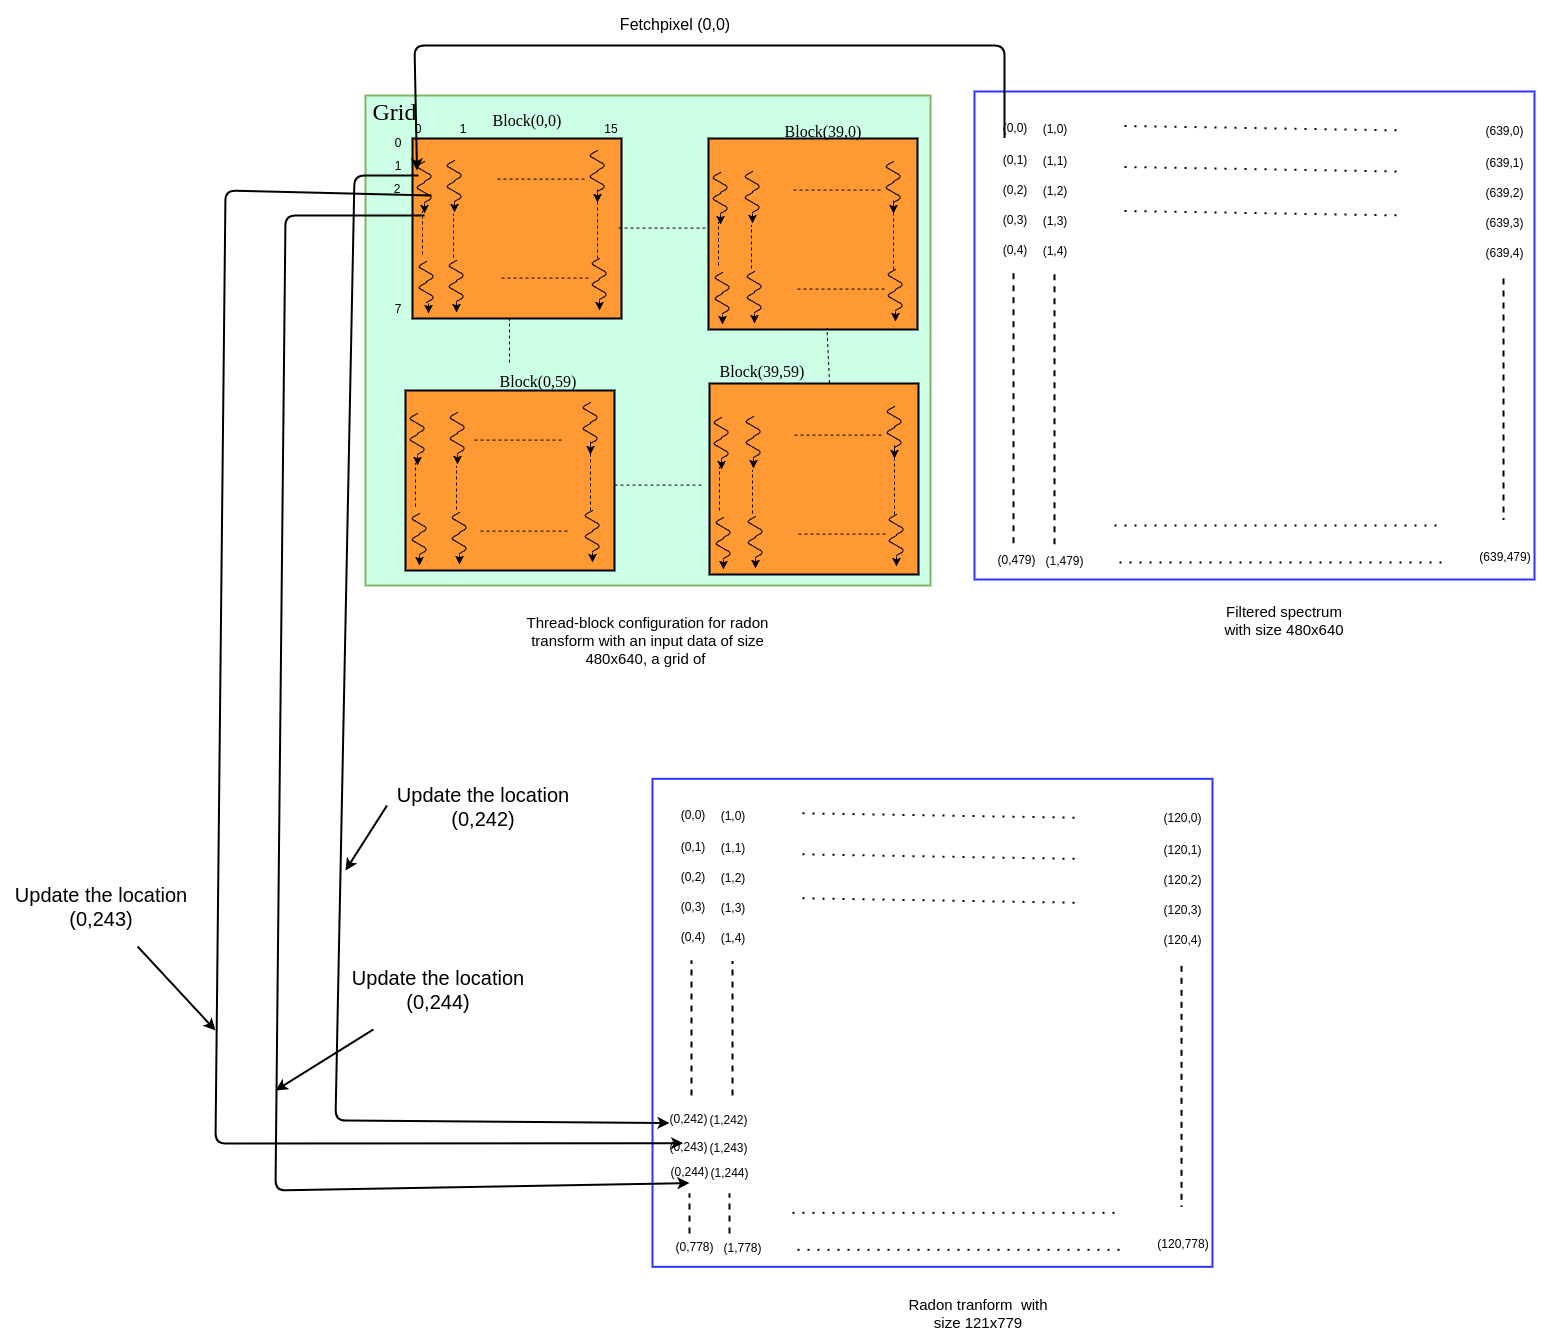
\includegraphics[width=0.75\linewidth]{radonThread.png}
	\caption{CUDA kernel for calculating Radon transform for a spectrum of size 640x480}
	\label{fig:radon threadaccess}
\end{figure}
\item \textbf{Blur length calculation} \hfill \break
The blur length calculation needs to find the target function as explained in the algorithm flow. The target function has different steps while calculating on GPU, they are explained below,
\begin{itemize}
	\item The input image is first converted into frequency domain. This can be done by using standard CUDA FFT library \textbf{cufft}, as shown in Figure \ref{fig:cufft}.
	\item Finding the magnitude and log transform are pixel parallel operations and does not depend on the other outputs. An output at location (u,v) can be produced by a single thread at (u,v) in the grid. For a spectrum of size 640x480 the output is also of same size. A block with 16x8 threads are found to be efficient, and a grid of 40x60 is created using equation \ref{grid-blockeq} to complete all the outputs.
	\item The result of log transform is rotated by blur angle. This data rotation is performed using OpenCV library on CPU and the blur calculation too implemented on CPU.
\end{itemize}
\end{itemize} 
\subsubsection{Deconvolution}
\begin{itemize}
	\item As explained in the algorithm, the deconvolution contains a series of convolutions explained in the Figure \ref{fig:Deconvolution flow chart}.
	\begin{figure}[h!]
		\centering
		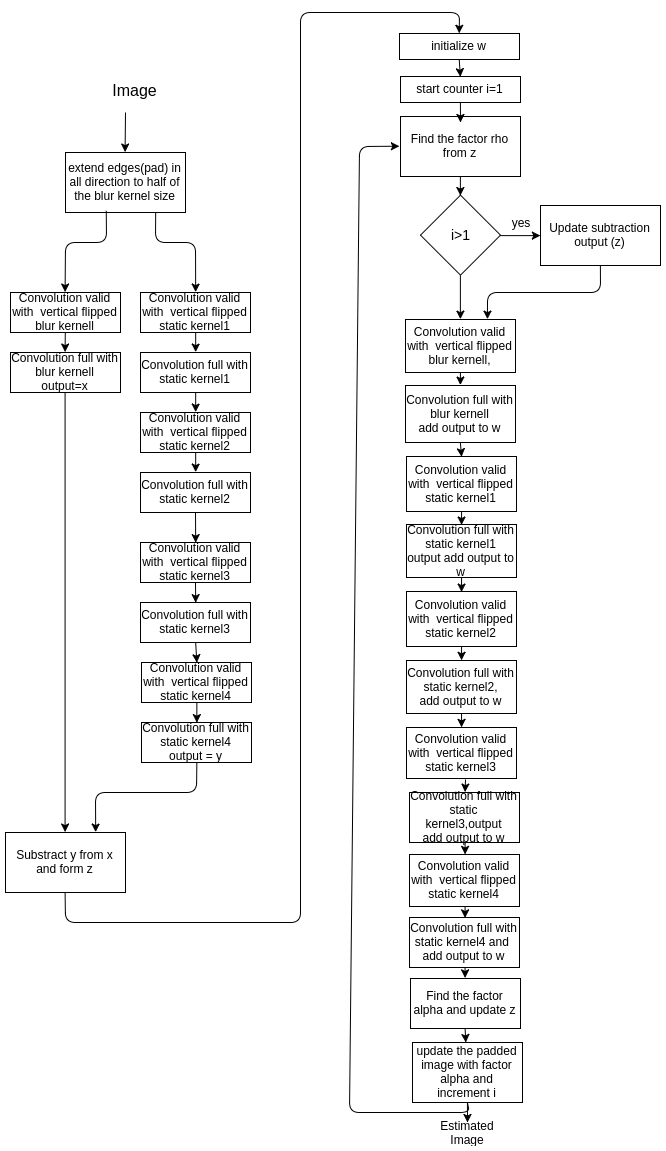
\includegraphics[width=0.8\linewidth]{deconvolutionflowchart.png}
		\caption{Sequence of operations in Deconvolution}
		\label{fig:Deconvolution flow chart}
	\end{figure}
	\item Initially the image is padded such that the boarders are extended by half kernel size. Its just a element wise copy operation. Single element copy operation can be handled by a single thread. 
	\item Creating a grid of threads with size equal to padded image then all the elements can be copied simultaneously. 16x16 threads for block considered in this case.
	\item For an image of 640x480 and a kernel with size 3x3 the output is 642x482. So a grid of 41x31 blocks is created using equation \ref{grid-blockeq} to complete the entire operation.
	\item The padded image is subjected to valid type of convolution with the flipped blur kernel. A window of pixels from the image multiplies with the respective elements from the blur kernel. The outputs from the multiplications are accumulated to form a single convolution output.
	\item If a thread can produce an output then the output size number of threads can generate all the outputs simultaneously. But each thread will iterate over multiple times, the iteration count is controlled by the size of kernel.
	\item A block with size 16x16 is considered for convolution operation. For the above padded image with size 642x482 needs 41x31 blocks to complete the entire convolution outputs.
	\item For the remaining types of convolutions, creating output size number of threads will complete the convolution operation.
	\begin{figure}[h!]
		\centering
		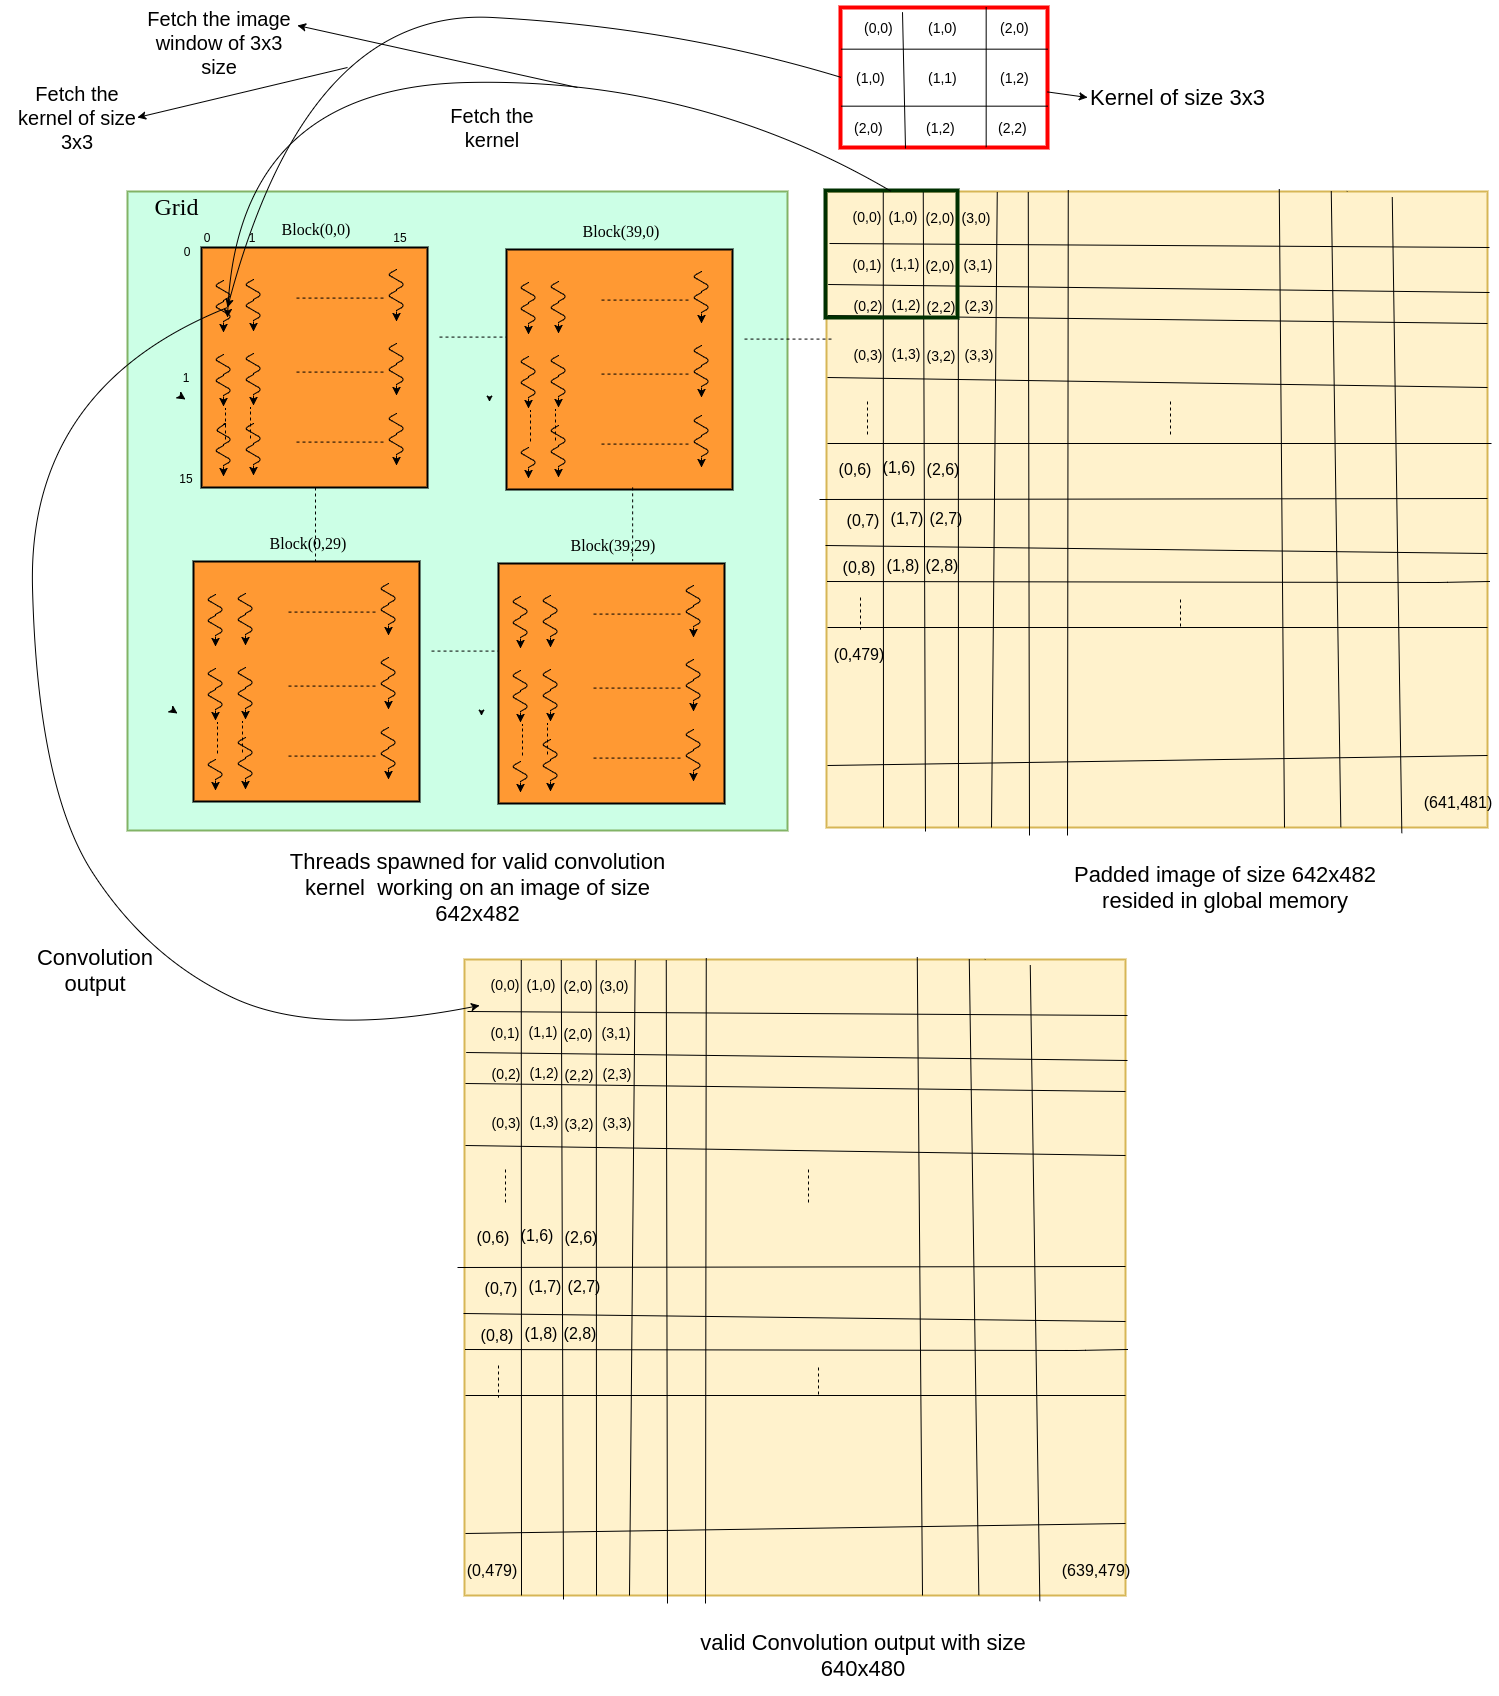
\includegraphics[width=\linewidth]{convolutionkernel.png}
		\caption{Valid type of convolution operation on GPU, thread access pattern. For an image of size 642x482 and a convolution kernel of size 3x3.}
		\label{fig:convolution kernel}
	\end{figure}
	\item For the remaining types of convolutions, creating output size number of threads will complete the convolution operations.
	\item The subtraction operation From the Figure \ref{fig:Deconvolution flow chart} is element wise. For inputs of size 642x482, this operation can be done on GPU with a grid of 41x31 blocks with 16x16 threads in block.
	\item Calculating factor $\rho$ and alpha needs to add all the elements from the output of subtraction operation. So \textit{atomicAdd} operations are used to add the elements.
\end{itemize}

\subsection{Results and discussions}
The motion de-blur algorithm is implemented on a CPU-GPU platform with Intel i5 CPU @3.0GHZ and a NVIDIA GeForce GT640 GPU with 384 CUDA cores. The algorithm is tested against images with different resolutions. The execution timing for each module are tabulated in Table \ref{table:motion de-blur}. This table also conatins the speed ups observed when compared to CPU only implementation. The speed up is calculated as the ratio of the CPU-GPU timing to the CPU only timing.

\begin{table}[htb]
	\centering
	\resizebox{\columnwidth}{!}{%
		\begin{tabular}{|m{6em}|m{1.0cm}|m{1.0cm}|m{1.0cm}|m{1.0cm}|m{1.0cm}|m{1.0cm}|}
			\hline
			\textbf{Module}&\multicolumn{2}{c|}{\textbf{CPU(in ms)}} & \multicolumn{2}{c|}{\textbf{GPU(in ms)}} &\multicolumn{2}{c|}{\textbf{Speed Up}} \\    \cline{2-7} 
			&\textbf{480p}&\textbf{1080p}&\textbf{480p}&\textbf{1080p}&\textbf{480p}&\textbf{1080p} \\    \hline
			Gradient of the image& 	14.50 & 90.94& 0.517& 2.32& 28x & 39x\\    \hline
			Power spectrum calculation& 18.24& 154.06& 1.26& 8.81& 17x& 19x \\   \hline
			Butterworth bandpass filtering	& 22.82& 135.29& 2.39& 3.72& 10x& 36x\\   \hline
			Radon transform & 16.52& 55.12& 3.85 & 12.05 & 4.3x& 4.5x \\   \hline	
			Deconvolution \newline&320.5&3246.99&29.86&29.86&11x&17x \\   \hline
			Total timing & 1600.50&4200.65&260.45&580.64&6x& 7x \\   \hline
		\end{tabular}}
		\caption{timing performance of motion de-blur algorithm}
		\label{table:motion de-blur}
	\end{table}
\begin{figure}[htb]
	{\centering
	\subfloat[input]{{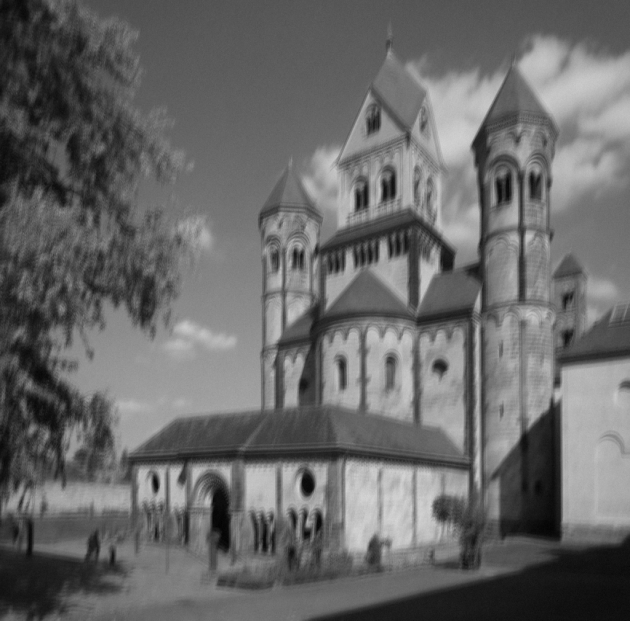
\includegraphics[width=6cm]{mdinput.png} }}%
	\qquad
	\subfloat[output]{{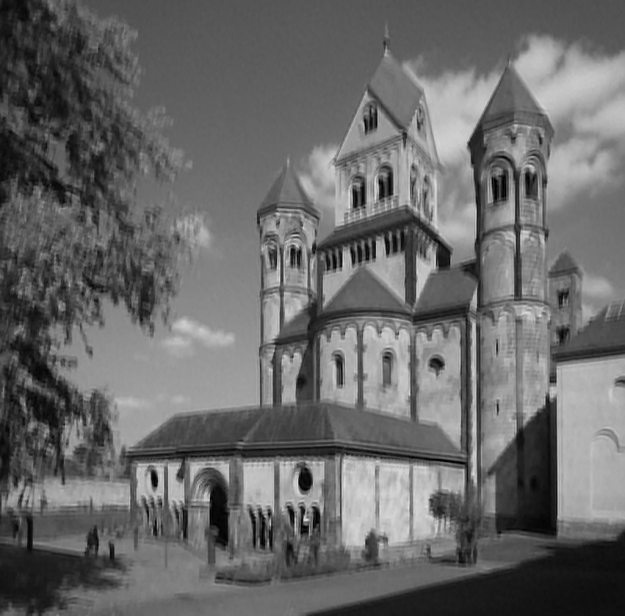
\includegraphics[width=6cm]{mdoutput.png} }}%
	\caption{Motion de-blur functional results}%
	\label{fig:motion de-blur results}%}
}
\end{figure}
\paragraph*{}From the Table \ref{table:motion de-blur} the module Radon transform speed up is low. This is because Radon transform uses atomicAdd operations for accumulating data in the projections. All the remaining modules are data parallel, thus a good speed up is observed in all these cases. All these speed up are observed without any use of texture or shared memory. Infact there is a possibility to use shared memory in some modules. The Gradient image works on two elements, in this current implementation those two are fetched from global memory, to save one memory transaction we can use shared memory. This can be applied to convolution kernel also where a window of pixels are used for a single output.


%\end{document}
